\chapter*{Appendix}\label{Sec:Appendix}

                \begin{figure}[ht]
                \begin{center}
                   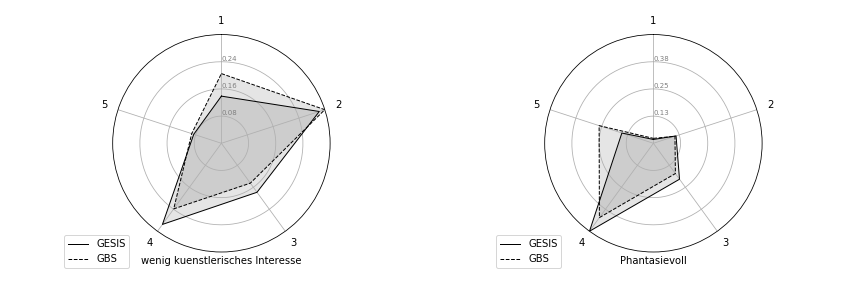
\includegraphics[scale=0.55,angle=0]{fig/Opennessfigure}
	         \label{Openness}
	         \caption{ Openness: \textit{" I see myself as someone who has few artistic interests"}(left). \textit{"I see myself as someone who has an active imagination"}(right).}
                \end{center}
                \end{figure}

                \begin{figure}[ht]
                \begin{center}
                   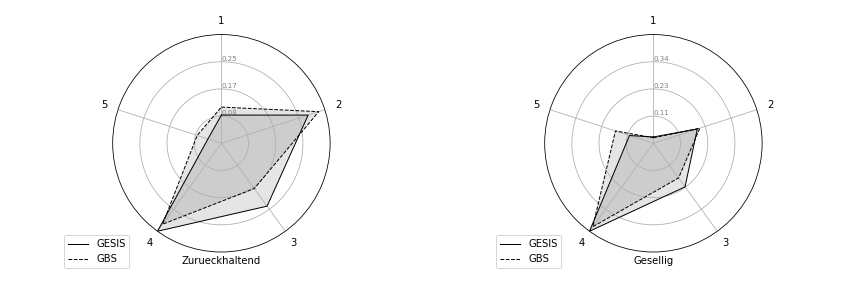
\includegraphics[scale=0.55,angle=0]{fig/Extraversionfigure}
	         \label{Extraversion}
	         \caption{Extraversion: \textit{"I see myself as someone who is reserved."}(left). \textit{"I see myself as someone who is outgoing, sociable. "}(right).}
                \end{center}
                \end{figure}

                \begin{figure}[ht]
                \begin{center}
                   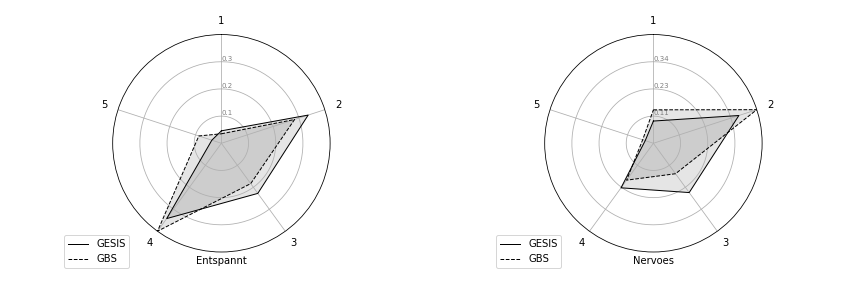
\includegraphics[scale=0.55,angle=0]{fig/Neuroticismfigure}
	         \label{Neuroticism}
	         \caption{Neuroticism: \textit{"I see myself as someone who is relaxed, handles stress well. "}(left). \textit{"I see myself as someone who gets nervous easily."}(right)..}
                \end{center}
                \end{figure}

\begin{figure}[H]
\begin{center}
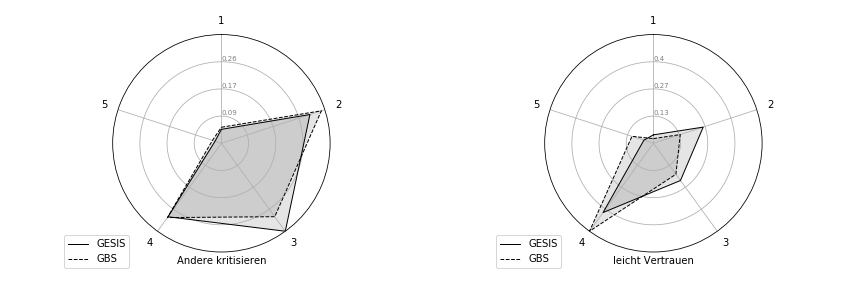
\includegraphics[scale=0.75,angle=0]{fig/Agreeablenessfigure}
\label{Agreeableness}
\caption{Agreeableness: \textit{""I see myself as someone who tends to find fault with others"}(left). \textit{"I see myself as someone who is generally trusting"}(right).}
\end{center}
\end{figure}